\documentclass[12pt,two column]{article}
\usepackage{amsmath}
\usepackage{graphicx}
\graphicspath{{Documents/}}
\newcommand{\myvec}[1]{\ensuremath{\begin{pmatrix}#1\end{pmatrix}}}
\let\vec\mathbf
\begin{document}
\title{ASSIGNMENT NO.1  \\COURSE CODE-AI1110\\ Probability And Random Variables }
\author{NAME-Abhishek Kumar ROLL NO.=AI21BTECH11003}
\maketitle
\section*{ Question 1a}
 Solve the following inequation and write down the solution set:\\
\begin{align}
 11x-4 < 15x+4\le13x+14\nonumber,  x\in \mathbb{W}\\\nonumber
\end{align}
Represent the solution on number line .
 \section*{Solution}
There are two inequatilities.\\
\begin{align*}
 11x-4 < 15x+4\le13x+14,  x\in \mathbb{W}\\
\end{align*}
Lets solve for left inequation.
\begin{align*}
 11x-4<15x+4\\
 \Rightarrow -8<15x-11x\\
 \Rightarrow-2<x\\
\end{align*}
 Lets solve for right inequation.\\
\begin{align*}
  15x+4\le13x+14\\
\Rightarrow 2x\le10\\
\Rightarrow x\le5\\
 -2 < x\le5,
x\in \mathbb{W}\\
\Rightarrow x=0,1,2,3,4,5 
\end{align*}
vector equations of lines:
\begin{align*}

 L1 \equiv 11x-4-y1=0\\
L2 \equiv 15x+4-y2=0\\
L3 \equiv 13x+14-y3=0\\

L1 \equiv \myvec{11 & -1} \vec{p}=4\\
\Rightarrow \myvec{11 & -1} \myvec{x \\ y1}=4\\
L2 \equiv \myvec{15 & -1} \vec{p}=-4\\
\Rightarrow \myvec{15 & -1} \myvec{x \\ y2}=-4\\
L3 \equiv \myvec{13 & -1} \vec{p}=-14\\
\Rightarrow \myvec{13 & -1} \myvec{x \\ y3}=-14\\  

y1=y2\\
\Rightarrow \myvec{11 & -1}\myvec{x\\1}=\myvec{15 & 4} \myvec{x \\ 1}\\
\Rightarrow -8=4x\\
\Rightarrow -2=x\\
y2=y3\\
\Rightarrow \myvec{15 & 4}\myvec{x\\1}=\myvec{13 & 14} \myvec{x \\ 1}\\
\Rightarrow 2x=10\\
\Rightarrow x=5\\
\end{align*}
MATRIX CALCULATIONS TO FIND \\INTERSECTION OF\\ L1 AND L2 ,L2 AND L3
\clearpage
\begin{figure}
THIS PLOT SHOWS LINES L1,L2,L3 INTERSECTING EACH OTHER
\includegraphics[scale=1]{figure_3.png}
\end{figure}
\clearpage
\begin{figure}
THE DOTS ARE THE POSSIBLE SOLUTIONS
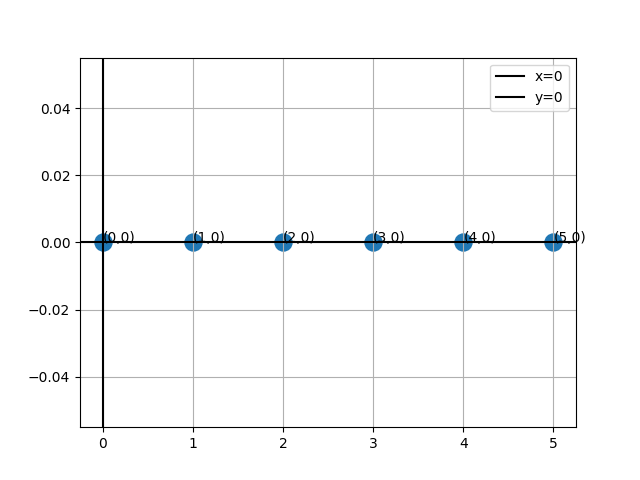
\includegraphics[scale=1]{Figure_4}
\end{figure}

\end{document}
